\documentclass{beamer}
\usepackage[english]{babel}
\usepackage[utf8]{inputenc}
\mode<presentation>{\usetheme{FS18}}
\usepackage{amsmath,amsthm, amssymb, latexsym}
\usepackage[orientation=portrait,size=a0,scale=1.4]{beamerposter}
\usepackage{natbib}
\usepackage{subcaption}
\graphicspath{{../figures/graphics/}}
 
\title{Applying a Reduced Model of Apical and Basal Dendritic Compartments to Sequence Learning in Recurrent Neural Networks}
\author{Fabian Schubert, Claudius Gros}
\institute{Institute for Theoretical Physics, Goethe University Frankfurt a.M.}
\date{Sept. 27th, 2018}

\renewcommand{\vec}[1]{\mathbf{#1}}

\newcommand{\vx}{\vec{x}}
\newcommand{\vy}{\vec{y}}
\newcommand{\vf}{\vec{f}}
\newcommand{\vsigm}{\boldsymbol{\sigma}}

\newcommand{\Err}{\mathrm{Err}}
\newcommand{\Exp}{\mathrm{E}}
\newcommand{\Var}{\mathrm{Var}}

\newcommand{\avg}[1]{\langle #1 \rangle}

\begin{document}
\begin{frame}[t]
\begin{columns}[t]
\begin{column}{.4\textwidth}
\begin{myblock}{Introduction}
\begin{itemize}
\item Experiments suggest that, depending on the amount of apical (distal) and basal dendritic synaptic drive, layer 5 pyramidal neurons can exhibit quietness, low frequency spiking and high frequency bursting \cite{Letzkus_2006,Shai_2015}.
\item High frequencies occur when distal and basal inputs coincide in time. A simplified, spiking compartment model of this effect has been used to gate plasticity of basal connections by means of distal synaptic inputs \cite{Bono_2017}.
\item In our framework, coincidence detection of distal and basal input modulates plasticity.
\item This error-driven learning could be used to extract a predictive signal from proximal connections.
\end{itemize}
\end{myblock}

\begin{myblock}{Model Description}
We used a discrete time rate encoding neuron model based on a phenomenological Layer 5 Pyramidal cell model by Shai et al. \cite{Shai_2015}, whose output frequency is given by
\vspace{1\baselineskip}
\begin{align*}
x\left(I_p,I_d\right) &= 2 \left[ \sigma\left(I_p-\theta_{p1}\right) \sigma\left(I_d-\theta_d\right)\ +\alpha\sigma\left(I_p-\theta_{p0}\right)\sigma\left(-\left(I_d-\theta_d\right)\right)\right] - 1 \\
\sigma\left(x\right) &= \frac{1}{1+\exp(-g\cdot x)} \\
I_p (t) &= \sum_{k=1}^{n_p} w_{p,k} (t) x_{p,k} (t) \\
I_d (t) &= \sum_{k=1}^{n_d} w_{d,k} (t) x_{d,k} (t) \\
\end{align*}
Proximal and distal weights were subject to the same form of Hebbian plasticity and weight normalization.
\vspace{1\baselineskip}
\begin{align*}
\Delta w_{i} (t) &= \epsilon_w \left(x(t)-\langle x \rangle\right)\left(x_{i}(t)-\langle x_{i} \rangle \right) \\
w_{i}(t+1) &= w_{\rm total} \frac{w_{i}(t) + \Delta w_{i}(t)}{\sqrt{\sum_{k=1}^{n} \left[ w_{pk}(t) + \Delta w_{pk}(t) \right]^2}}
\end{align*}
\end{myblock}

\begin{figure}
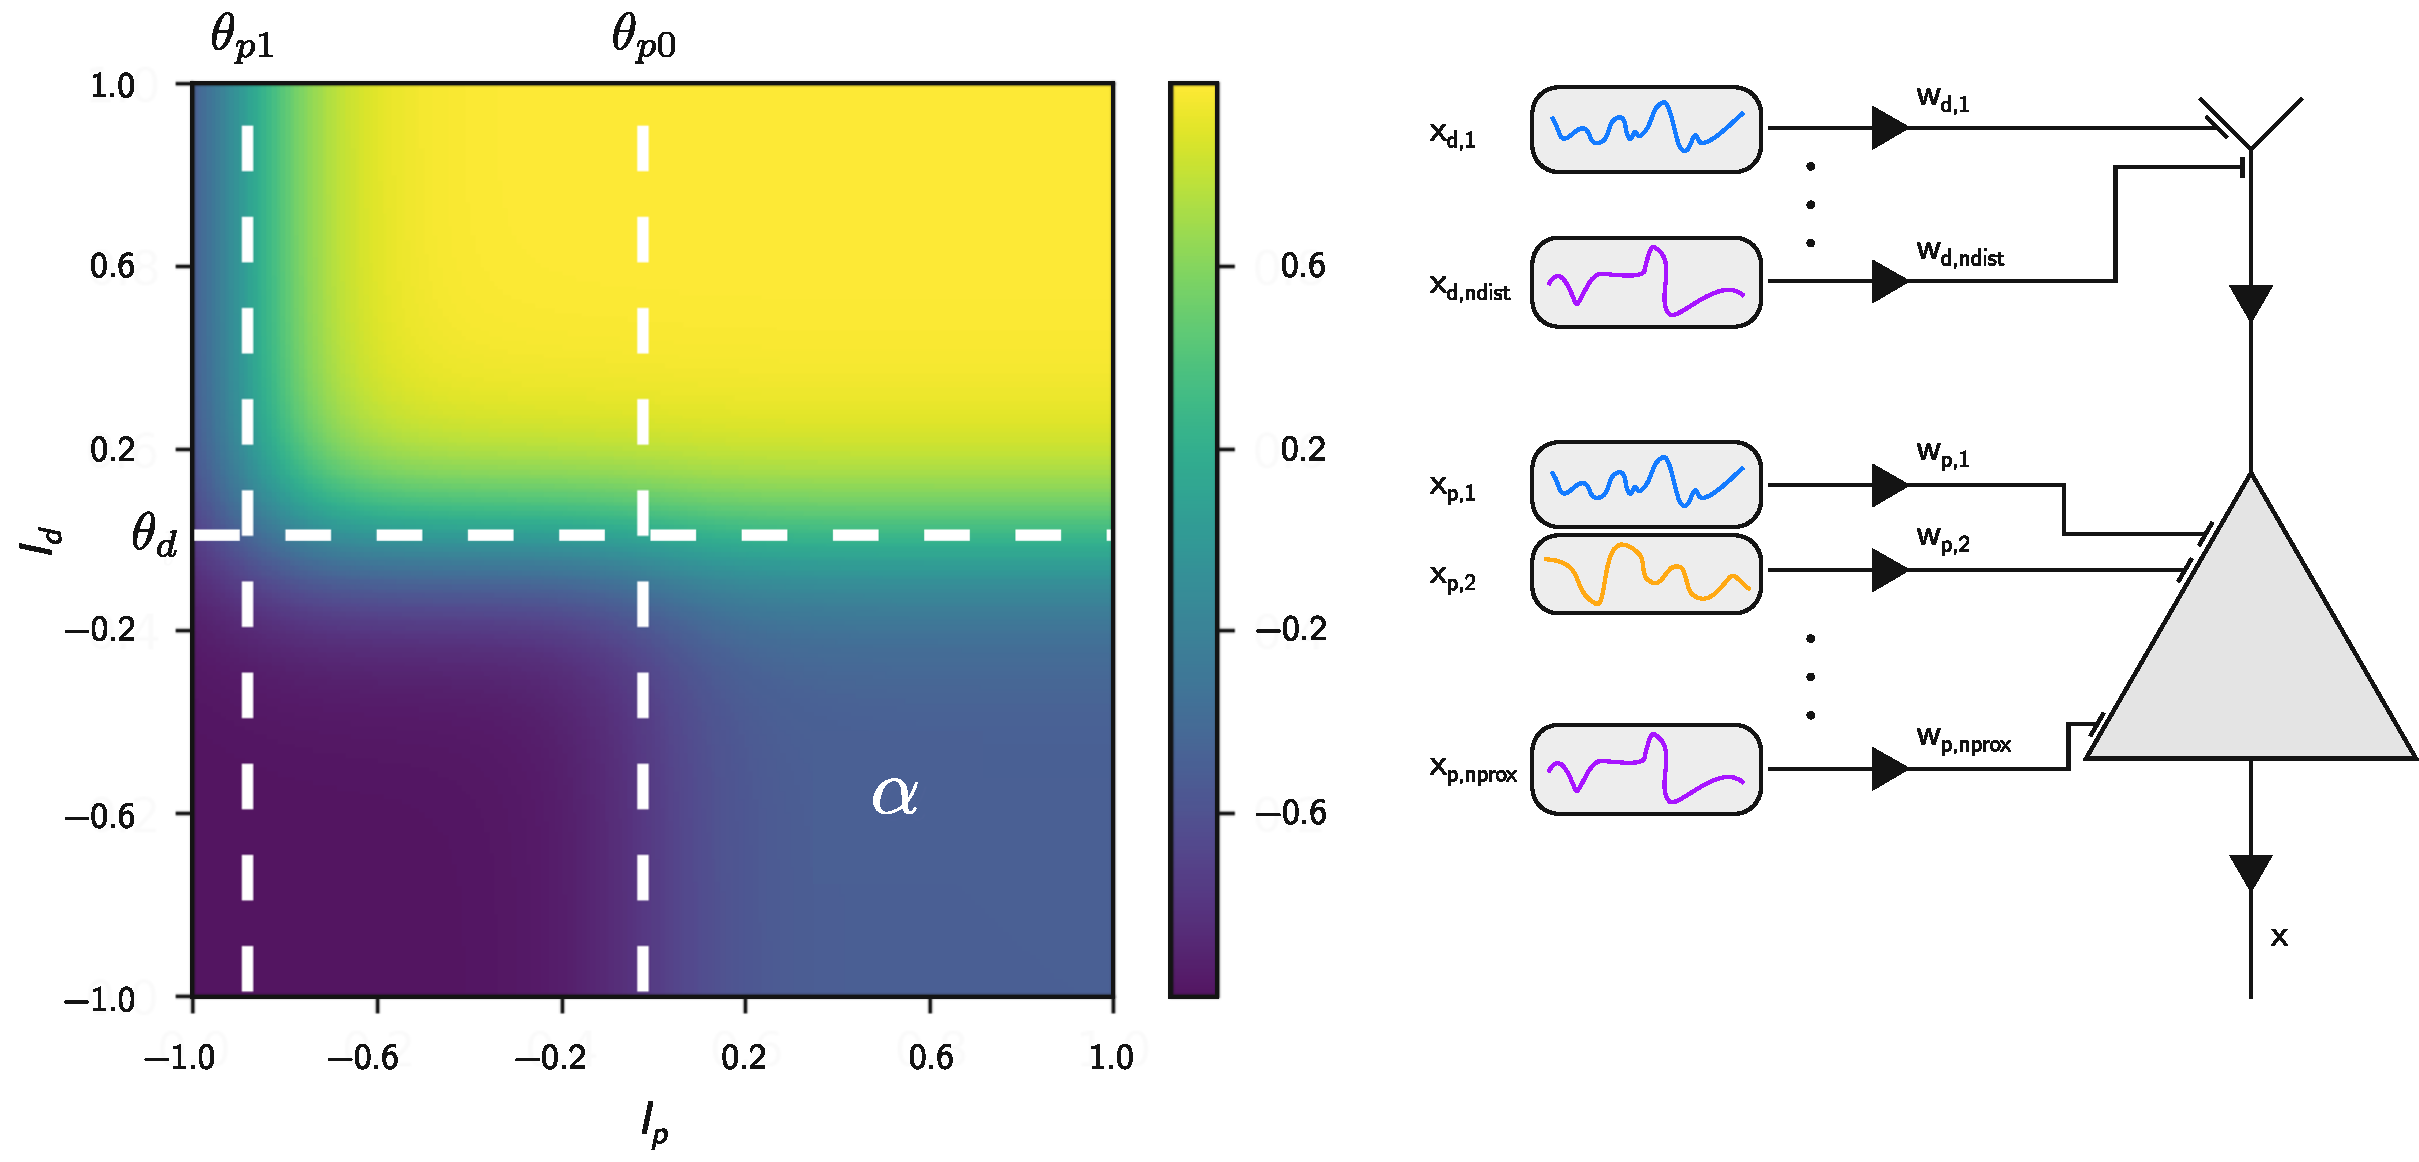
\includegraphics[width=\textwidth]{../figures/fig1.pdf}
\caption{Left: Output rate as a function of proximal (basal) and distal (apical) dendritic input. Right: Illustration of the accumulation of inputs in the neuron model. $\alpha$ denotes the low-frequency rate.}
\label{fig:Model_Illustration}
\end{figure}


\end{column}

\begin{column}{.5\textwidth}
\begin{myblock}{Results for a Single Neuron}
\begin{itemize}
\item We fed a single neuron with 10 randomly fluctuating proximal inputs and one distal input that was exactly correlated with one of the proximal signals. 
\item As a ``distraction", the standard deviation of another proximal input was increased, giving the proximal inputs had a dominant principal component.
\item As shown in Fig.~\ref{fig:Results_1}, the distal input acts as a guiding input, such that plasticity potentiates the proximal input that maximizes correlation with the distal input, in spite of the distracting signal.
\item If the distal input is uncorrelated with any of the proximal input, proximal weights select the principal component.
\item Learning of multiple distal inputs is dominated by the principal component.
\end{itemize}
\end{myblock}

\begin{myblock}{Analytic Approximation}
An analytic approximation of the proximal weight dynamics consists of two dominant terms, containing the proximal covariance matrix and proximal-distal covariances.
\begin{align*}
\Delta w_{p,i} &\approx \epsilon'_w \sum_j \alpha C^{xx}_{ij} + (2-\alpha) C^{dx}_i \\
C^{xx}_{ij} &\equiv \avg{\left(x_i - \avg{x_i} \right)\left( x_j - \avg{x_j} \right)} \\
C^{dx}_i &\equiv \avg{\left(d - \avg{d} \right) \left(x_i - \avg{x_i} \right)} \\
\epsilon'_w &\equiv \epsilon_w \frac{g}{8}
\end{align*}
\end{myblock}

\begin{myblock}{Coupling with an Echo State Network for Sequence Prediction}
\begin{itemize}
\item We hypothesized that a single unit sending its output to a random Echo State network while also receiving proximal input from the same reservoir, the neuron could learn to predict the guiding signal fed in as a distal input, as illustrated in Fig.~\ref{fig:Results_4}.
\item In contrast to the usual Echo State architecture, input and output are merged into a single unit.
\item Prediction of the guiding signal succeeded if the learning rule was modified such that it included a local error signal:
\end{itemize}
\begin{equation*}
\Delta w_{d,i}(t) = \epsilon_w \left(I_p(t)-I_d(t)\right) x_{d,i}
\end{equation*}
\begin{itemize}
\item After learning, the proximal input acted as a predictor of the distal guiding signal, see Fig.~\ref{fig:Results_4}.
\item Compared to separate input and output units, the convergence of the learning process was prolonged, since the input signal was disturbed by the initially random proximal input.
\end{itemize}
\end{myblock}



%\begin{figure}
%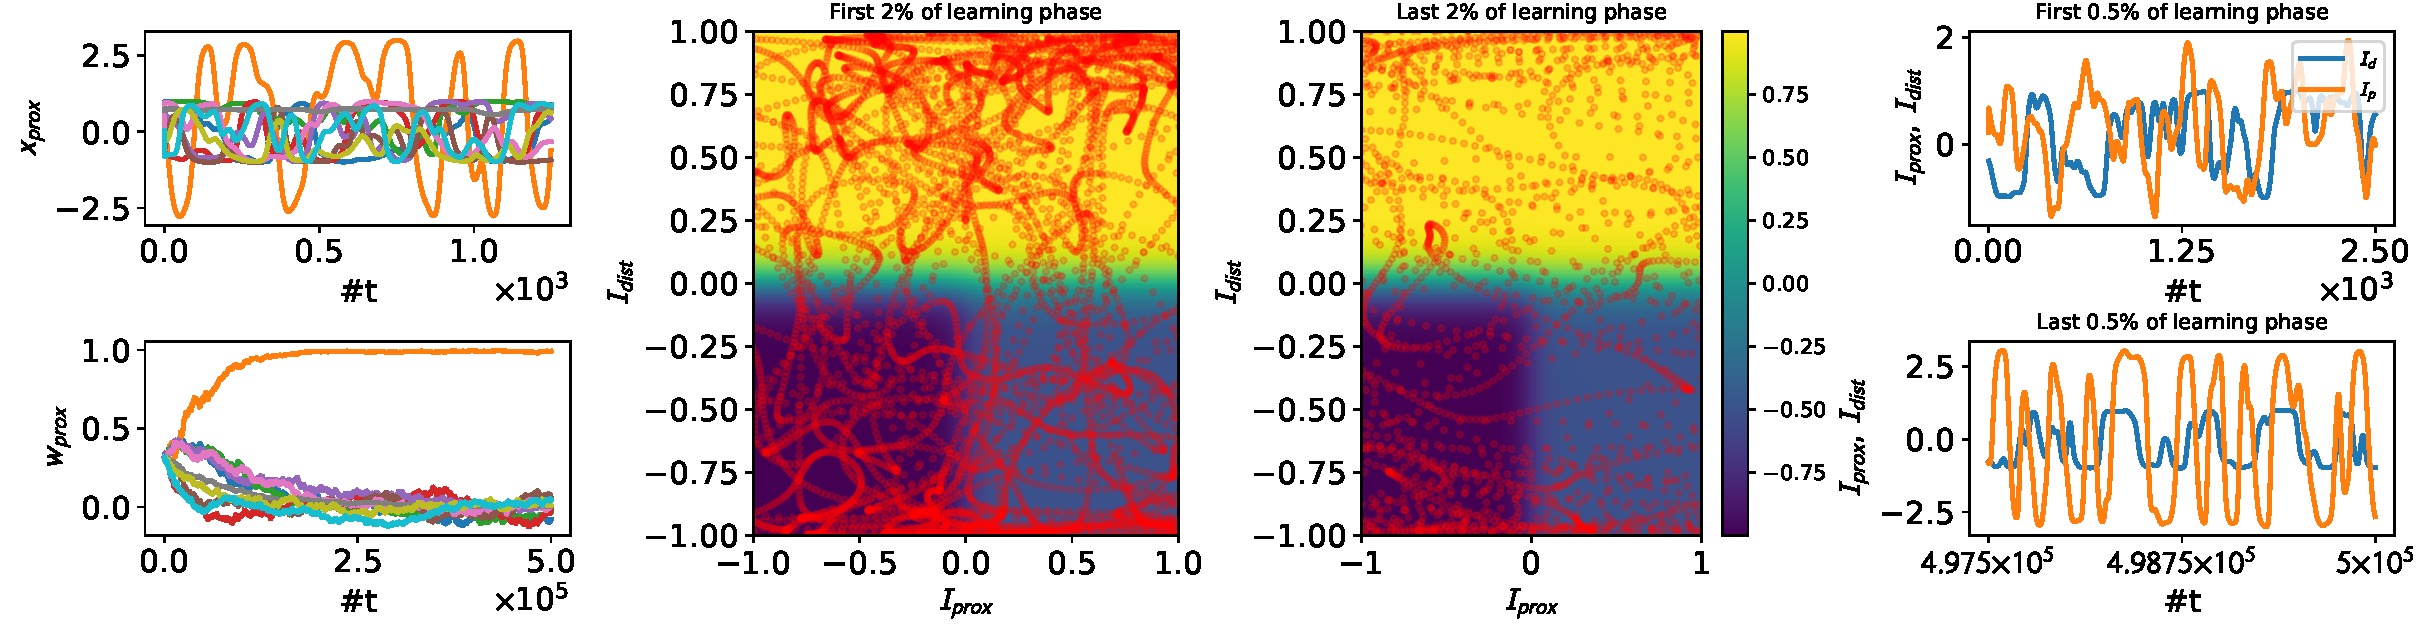
\includegraphics[width=\textwidth]{../figures/fig3.pdf}
%\caption{Single distal input, uncorrelated}
%\label{fig:Results_2}
%\end{figure}



%\begin{figure}
%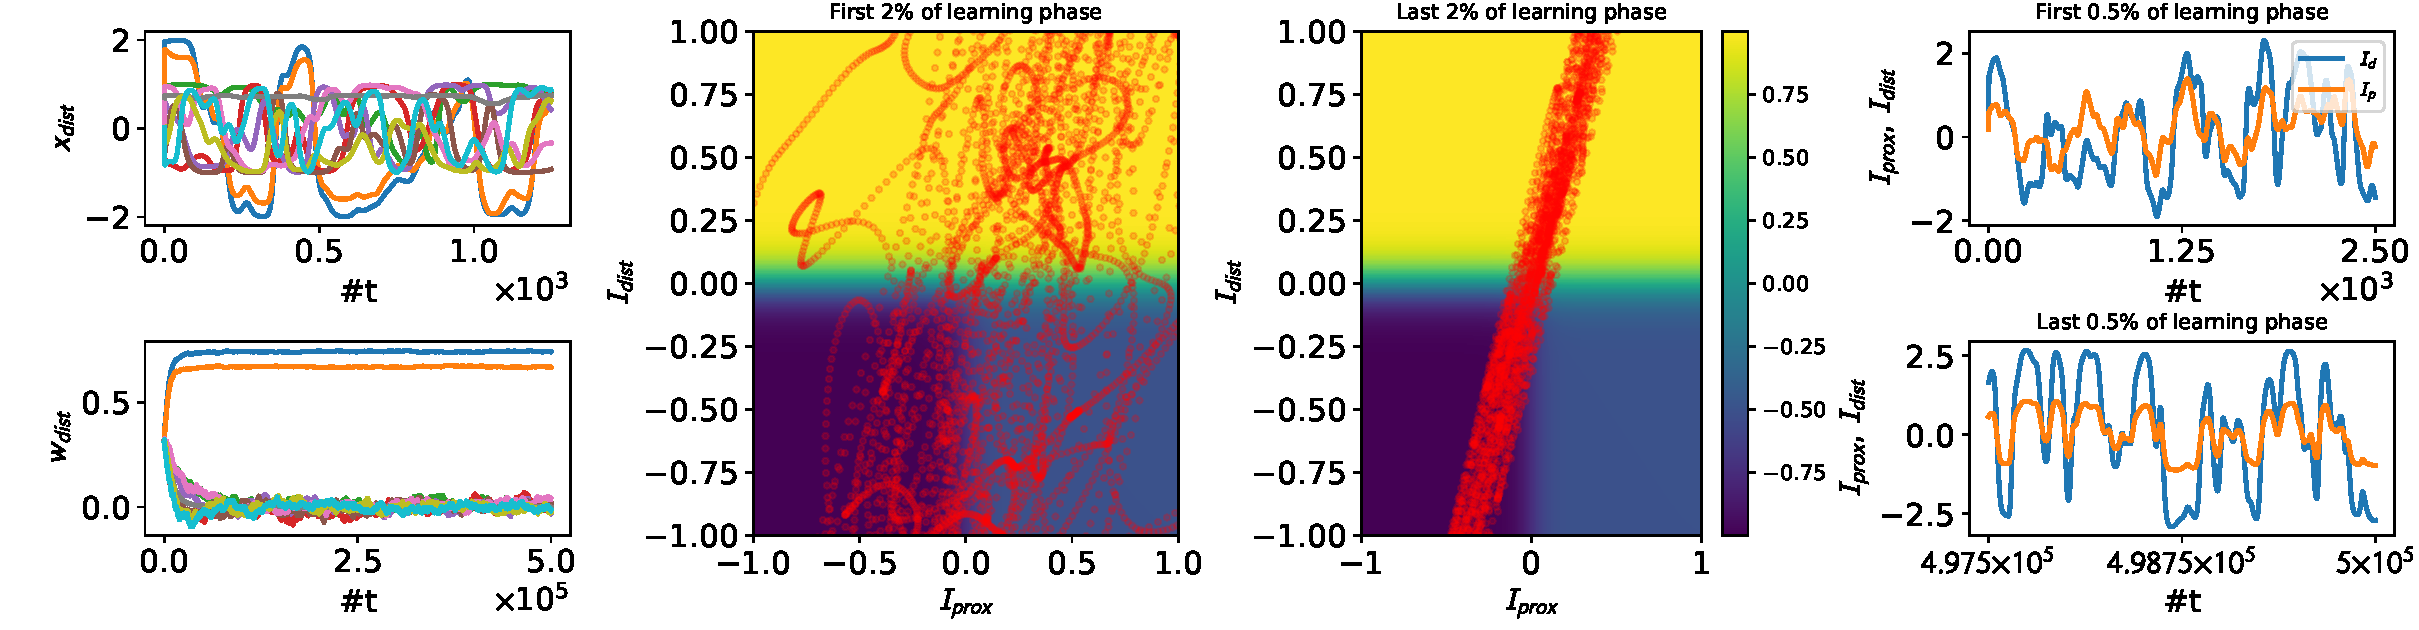
\includegraphics[width=\textwidth]{../figures/fig4.pdf}
%\caption{Learning of principal component in the distal inputs.}
%\label{fig:Results_3}
%\end{figure}

\begin{figure}

\begin{subfigure}{0.3\textwidth}
\centering
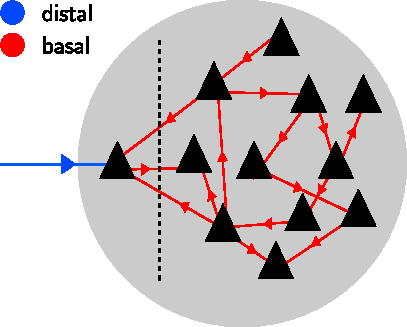
\includegraphics[width=\textwidth]{../figures/illustration_echo_state.pdf}
\end{subfigure}
\begin{subfigure}{9.5in}
\centering
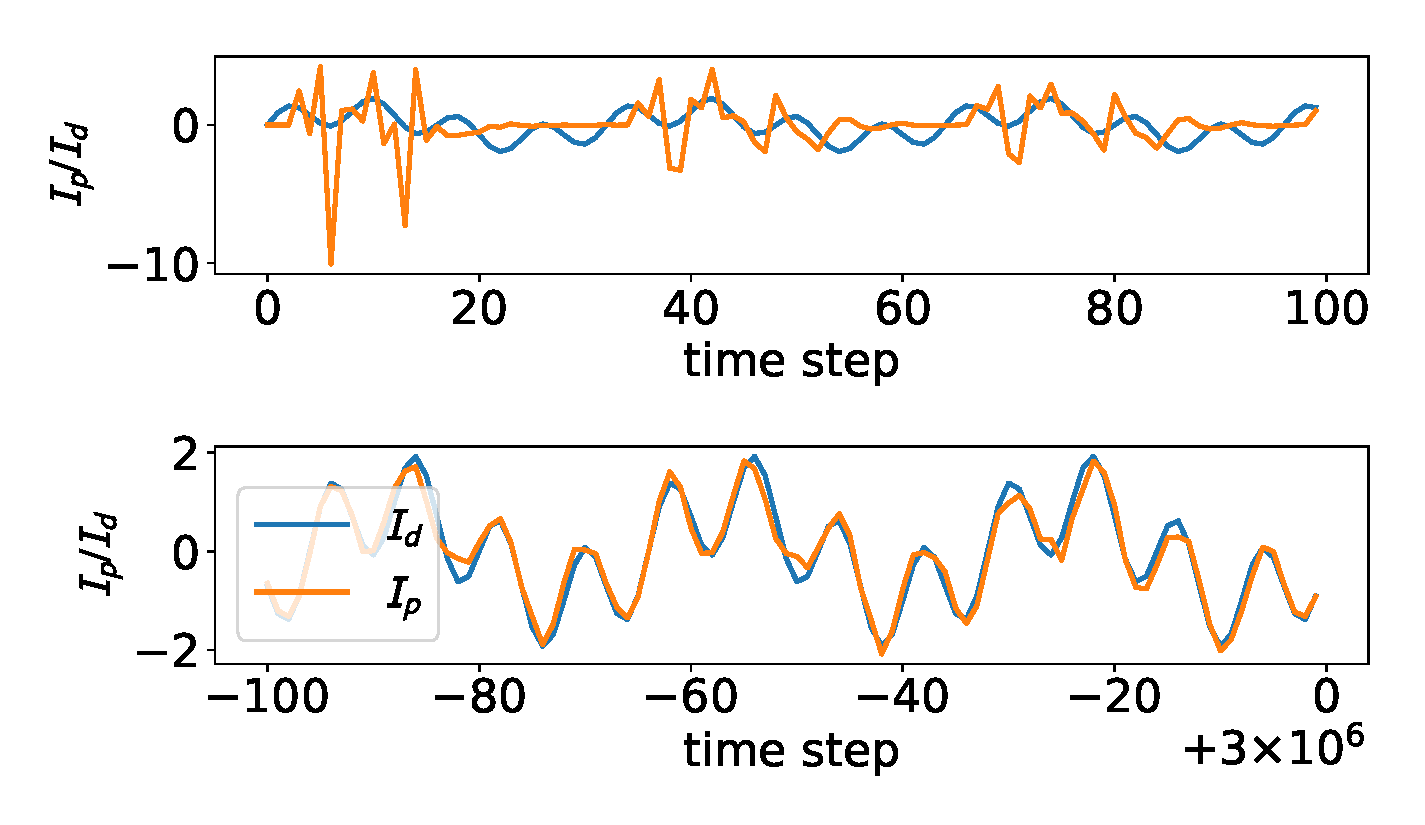
\includegraphics[width=\textwidth]{../figures/fig4_right.pdf}
\end{subfigure}
\caption{Combining the neuron model with an Echo State network for sequence prediction.}
\label{fig:Results_4}
\end{figure}

\end{column}
\end{columns}
\vspace{\baselineskip}
\begin{figure}
\begin{flushleft}
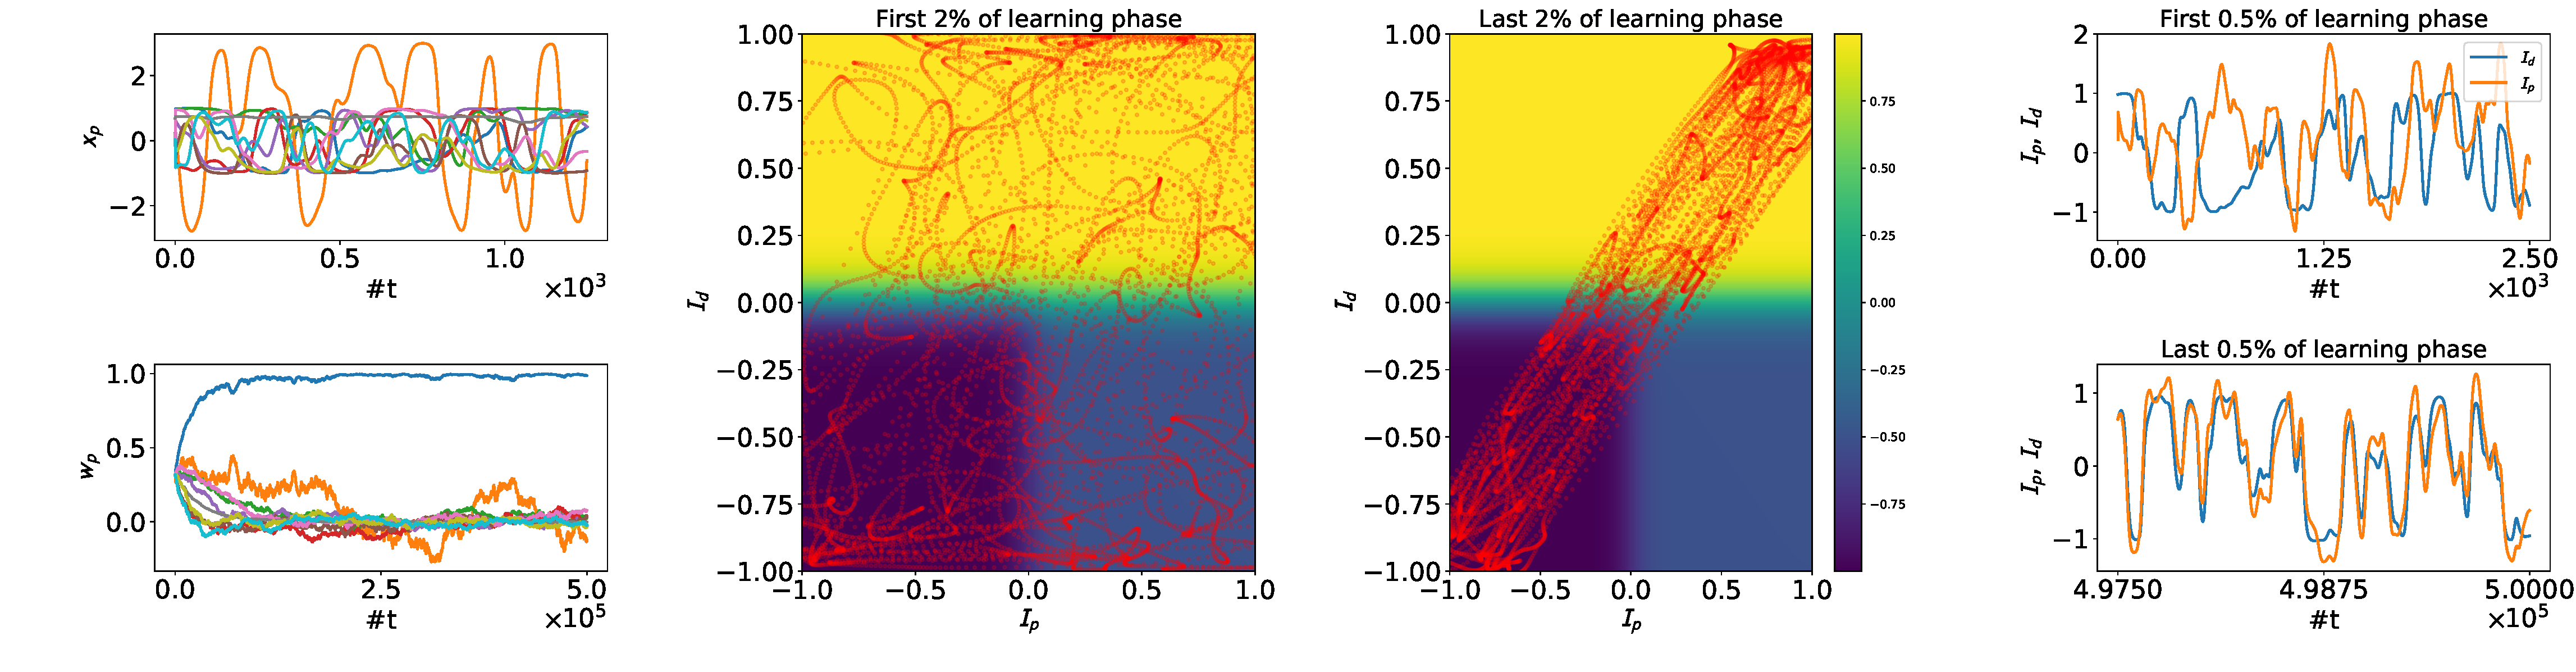
\includegraphics[width=0.95\textwidth]{../figures/fig2.pdf}
\end{flushleft}
\caption{Results for a single distal input, correlated with one proximal input}
\label{fig:Results_1}
\end{figure}

\begin{columns}[t]
\begin{column}{.4\textwidth}
\vspace{-1.83\baselineskip}
\begin{myblock}{Conclusions}
\begin{itemize}
\item The specific activation function of our model neuron acts as a coincidence detector between proximal and distal inputs.
\item This property can gate plasticity, where the distal input acts as a guiding signal.
\item We hypothesize that this property can be used in a predictive framework, e.g. by means of a recurrent, proximally connected dynamic reservoir.
\item Future work: Can external proximal input be included? If so, can we extend this model to a hierarchical predictive structure?
\end{itemize}
\end{myblock}
\end{column}
\begin{column}{.5\textwidth}
\noindent\rule{\textwidth}{2px}
\begin{footnotesize}
\bibliographystyle{unsrt}
\bibliography{poster_citations}
\end{footnotesize}
\end{column}
\end{columns}

\end{frame}
\end{document}
